\documentclass{article}
\usepackage{graphicx}
\usepackage{amsmath}
\author{Lukas Kohlhase}
\title{Demonstration of capabilities of tex2word and tex2docx}
\begin{document}
\maketitle
\tableofcontents
\section{General Text formatting}
\subsection{Playing around with bold and italic}
Normally formatted text looks like this. \footnote{Footnotes are also possible. \textbf{Markup in footnotes works as well}} \textbf{Common text formatting is supported, just as you would expect. \textit {Nested bold and italic works as well}}. Note that the width of a line is larger in Word than in the default LaTeX uses.  \\ 
\subsection{A normal paragraph again}
New paragraphs are back to the default. Since every kind of text formatting has to be manually added to the xslt files, just contact me (l.kohlhase@jacobs-university.de) if your text formatting doesn't work. 
\subsection{Lists}
\begin{enumerate}
\item item1
\begin{enumerate}
\item nested item 1
\item nested item 2
\end{enumerate}
\item item 2 
\item item 3 \ldots 
\end{enumerate}
Note that I haven't been able to make itemize lists work with showing dots instead of numbers. At the moment all lists are enumerated.
\subsection{Errors}
Errors are printed in red. If the output is simply Error: nameoftag , then this probably means that LaTeXML did not recognize your macro. \\ 
If it says the stylesheet did not recognize the element then this is an error in the stylesheet and you should contact me (l.kohlhase@jacobs-university.de) so that I can add the appropriate things to the stylesheets. 
\subsection {Tables}
\begin{tabular}{ c c c }
  1 & 2 & 3 \\
  4 & 5 & 6 \\
  7 & 8 & 9 \\
\end{tabular}
Everything should work here, but sometimes there is trouble with nested tables. 

\section{mathematics}
All kinds of mathematics is able to be displayed. \\ 
Inline math works, $a^2+b^2=c^2$, but as in TeX be careful with the bigger ones, they might look weird $\sum\limits_{k=0}^{\infty} \frac{x^k}{k!} =e$ \\
Note that the limits of the sum are not at the correct places, even though I used \textbackslash limits . \\ 
Display math: 
\[
\sum\limits_{k=0}^{\infty} \frac{x^k}{k!} =e
\]
And everything looks proper again. However there are still some slight differences that are inherent to the different ways of representing math. \\
Equations look like this
\begin{equation}
a^2+b^2=c^2
\end{equation}
The align environment looks like this: 
\begin{align}
a^2+b^2&=c^2&=\frac{E}{m} \\ 
&=26 &=123
\end{align}
Evidently this does not work well. This is an issue with the transformation of MathMl to OMML (word math format) that I am not in a position to fix. 
\section{pictures}
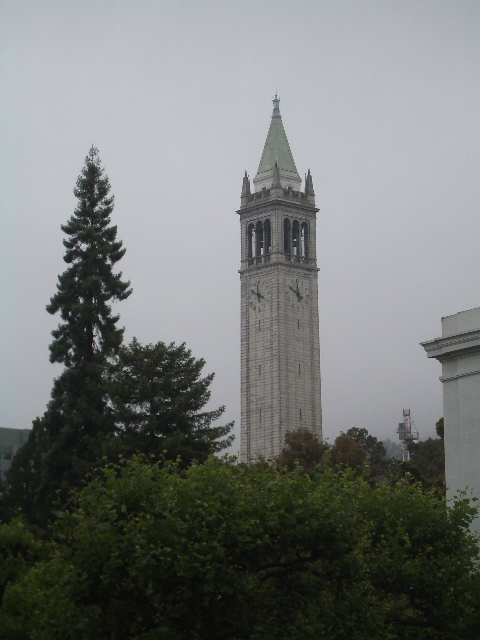
\includegraphics{image1}
Including graphics works as well. Note that the only supported formats at the moment are jpeg, png and eps. Graphics need to be kept in the same directory as the .tex file or in one of its subdirectories.  \\ 

Figures etc. Work, however captions are not supported at the moment. 
\section{references}
\cite{book1} \cite{book2} \cite{booklet1,incollection1} \cite{inbook1} \cite{inproceedings1} \cite{mastersthesis1} \cite{phthesis1} \cite{manual1} \cite{misc1} \cite{proceedings1} \cite{unpublished1}
Note that when first opening these references and using --profile=word, they are not formatted yet and only appear as numbers. To change the citation style, go to the references tab and then change the style in the style selector. Standard LaTeX References have the style IEEE 2006.  \\ 
Note that the bibliography is not added by default if you used --profile=word . In this case you again go to the references tab, click on Bibliography and then on Works cited to insert it yourself. 
\bibliographystyle{alpha}
\bibliography{test}
\end{document}
